
\clearemptydoublepage
\chapter{Discussion d'extension des résultats}
\label{chap:discussion}

\begin{quote}
    Closure. I keep hearing that word. $[...]$ As soon as a show has a sense of closure, it gives you an excuse to forget you've seen the damn thing.

    \hfill%
    David Lynch, 1990\footnote{\url{https://web.archive.org/web/20200805032143/https://www.latimes.com/archives/la-xpm-1990-02-18-ca-1500-story.html}}
\end{quote}



Ce chapitre présente un éventail de pistes de réflexions, d'extensions des résultats sur les problèmes à relaxation rapide du chapitre précédent. Rappelons d'abord le contexte: on considère la solution~$t \mapsto u^\eps(t)$ du problème
\begin{equation} \label{ext:pb:u}
    \pa_t u^\eps = -\frac{1}{\eps}A u^\eps + f(u^\eps),
    \qquad
    u^\eps(0) = u_0 \in \setR^d
\end{equation}
avec $A$ une matrice diagonale positive à valeurs propres entières, et $u \mapsto f(u)$ un champ de vecteurs régulier. Pour tout ordre $n \in \setN$, on construit un changement de variable $(\tau, u) \mapsto \Omega\rk n _\tau (u)$ proche de $e^{-\tau A}$ et un champ de vecteurs non-raide $u \mapsto F\rk n (u)$. Cela permet de décomposer la solution $t \mapsto u^\eps(t)$ en une partie \textit{macro} $v\rk n(t)$ et une partie \textit{micro} $w\rk n(t) = \bigO(\eps^{n+1})$, de sorte que 
\begin{equation} \label{ext:eq:decomp}
    u^\eps (t) = \Omega\rk n _{t/\eps} \big( v\rk n (t) \big) 
        + w\rk n (t) .
\end{equation}
Le problème micro-macro sur $(v\rk n, w\rk n)$ s'écrit 
\vspace*{-12pt}
\begin{subequations} \label{ext:pb:vw}
    \renewcommand{\arraystretch}{1.4}
    \begin{empheq}[left=\empheqlbrace]{align}
    &\dpt v^{[n]}(t) = F^{[n]}(v^{[n]}) ,
    \label{ext:pb:v}
    \\ \displaystyle
    &\dpt w^{[n]}(t) = - \inveps A w^{[n]} 
    + f\left( \Omega^{[n]}_{t/\eps}(v^{[n]}) + w^{[n]} \right) 
    - f\left( \Omega^{[n]}_{t/\eps}(v^{[n]}) \right) 
    - \eta^{[n]}_{t/\eps}(v^{[n]}),
    \label{ext:pb:w}
    \end{empheq}
\end{subequations}
avec $\eta\rk n$ le défaut définit par
\begin{equation} \label{ext:def:eta}
    \eta\rk{n}_{\tau} = 
    \frac{1}{\eps}\left( \dptau +  A \right) \Omega^{[n]}_{\tau} 
    + \dpu \Omega^{[n]}_{\tau} \cdot F^{[n]} - f \circ \Omega^{[n]} . 
\end{equation}
La donnée initiale est $v\rk n (0) = \big( \Omega\rk n _0 \big)^{-1} (u_0)$, $w\rk n (0) = 0$. Ce problème est bien posé et on peut le résoudre avec une \textit{précision uniforme} à l'ordre $n+1$ en utilisant un schéma exponentiel Runge-Kutta. 

Dans ce chapitre, on discute de quelques sujets ouverts qui pourraient faire l'objet d'études futures. En particulier, en Section~\ref{ext:sec:direct} on discute de problématiques d'implémentation, comme le coût de calcul, l'accumulation d'erreurs, et le besoin d'une dérivée exacte. En Section~\ref{ext:sec:auto} on définit un problème micro-macro autonome, ce qui permet d'expliquer le gain d'ordre remarqué en fin de Chapitre~\ref{chap:dissip-mima} et de définir une approche~\enquote{pullback} comme ce qui avait pu être fait dans le cadre hautement oscillant. Enfin en Section~\ref{ext:sec:telegraphe}, on présente une piste basée sur des développements de Padé pour traiter l'équation du télégraphe de manière rigoureuse à tout ordre. 


\section{Extensions directes du micro-macro}
\label{ext:sec:direct}

On présente ici des problématiques d'implémentation et de coût numérique, ainsi qu'une piste d'extension possible pour rendre le développement micro-macro automatique.


\subsection{Problématiques numériques}

Avec notre construction micro-macro, les non-linéarités du problème sont exacerbées. Par exemple sur le problème

\begin{equation*} 
    \left\lbrace\begin{array}{ll} \displaystyle \vphantom{\int}
      \dot x = g(x) - z , 
      & x(0) = u(0) , \\ \displaystyle
      \dot z = -\frac{1}{\e} z + g'(x) \big( g(x) - z \big) ,
      & z(0) = g(u(0)) - \tilde{u}(0) .
    \end{array}\right.
\end{equation*}
avec $g(x) = x^3/3$, on a implémenté (en Julia) le défaut à l'ordre 2 de la manière suivante:


\begin{lstlisting}
function eta2(x,z,epsil)
    etaXCoeffs = [
        64*x^12*z/9 + 8*x^6*z^3/3 ;
        88*x^10*z/9 + 4*x^4*z^3 ;
        68*x^8*z/9 + 4*x^5*z^2 + 2*x^2*z^3 ;
        6*x^6*z + 4*x^3*z^2 + z^3/3 ;
        13*x^4*z/3 - x*z^2 ;
        0 ;
        0
    ]
    etaZCoeffs = [
        -32*x^10*z^5/3 ;
        -80*x^8*z^5/3 ;
        -80*x^9*z^4/3 - 80*x^6*z^5/3 ;
        -160*x^7*z^4/3 - 40*x^4*z^5/3 ;
        -160*x^11*z^2/9 - 80*x^8*z^3/3 - 32*x^5*z^4 - 10*x^2*z^5/3 ;
        -52*x^9*z^2/3 - 40*x^6*z^3 - 16*x^3*z^4/3 - z^5/3 ;
        -448*x^13/81 - 268*x^7*z^2/9 - 16*x^4*z^3 + x*z^4/3 ;
        -32*x^11/9 - 59*x^5*z^2/3 - 10*x^2*z^3/3 ;
        -95*x^9/27 - 26*x^3*z^2/3 - z^3 ;
        0 ;
        0
    ]
    etaX, etaZ = BigFloat(0), BigFloat(0)
    for xCoeff in etaXCoeffs
        etaX = epsil*etaX + xCoeff
    end
    for zCoeff in etaZCoeffs
        etaZ = epsil*etaZ + zCoeff
    end
    return [etaX;etaZ]
end
\end{lstlisting}
%
Cette implémentation voit $\eta\rk n(x,z)$ comme un polynôme en $\eps$ et applique la méthode d'Horner (voir~\cite[Sec.~4.6.4]{knuth.2014.art}), ce qui permet d'avoir un résultat pertinent dans le cas où $\eps^2$ est proche de l'erreur machine. 

On voit cependant apparaître des termes jusqu'à $x^{13}$, ce qui peut vite être problématique du point de vue de la stabilité numérique, dès lors que $x$ prend des valeurs élevées. Sur le problème d'origine, la non-linéarité est cubique seulement, et $g(5) \leq 100$, donc on pourrait choisir $x(0) = 5$ dans le problème d'origine sans s'inquiéter de problèmes d'erreur numérique. Cependant, on a alors $x^{13} \sim 10^9$, ce qui peut engendrer des erreurs importantes dans le calcul du défaut, surtout si~$\eps$ est grand. On peut voir cela comme une illustration de la condition de bonne-définition des développements, 
\begin{equation*}
    (n+1) \eps \leq \frac{\rho}{\sup_{|v| \leq \rho} |f(u+v)|}
\end{equation*}
avec $n$ l'ordre du développement. 

En outre, une évaluation de $\eta\rk n (x,z)$ avec l'implémentation ci-dessus demande 24.5~$\mu$s, ce qui est 35 fois supérieur aux 699~ns que demande une évaluation du champ de vecteurs d'origine $f(x,z) = \left(\frac{1}{3}x^3 - z \right) \among{1}{x^2}$. Il paraît donc évident qu'une fois la phase transitoire passée, il vaut mieux utiliser un schéma \enquote{UA à l'équilibre} sur le système d'origine pour éviter les calculs coûteux.



\subsection{Dépasser les développements formels}

Dans le Chapitre~\ref{chap:dissip-mima}, la décomposition micro-macro est construite \textit{via} des résolutions successives de l'équation homologique
\begin{equation}
    \pa_\tau \Omega\rk{n+1} _\tau + A\Omega\rk{n+1} _\tau
    = \eps \left( 
        f \circ \Omega\rk n _\tau 
        - \pa_u \Omega\rk n _\tau \cdot F\rk n 
    \right) .
\end{equation}
On utilise donc des outils de calcul formel pour construire les applications~$(\tau, u) \mapsto \Omega\rk n _\tau(u)$ et $u \mapsto F\rk n (u)$ \textit{a priori} de l'implémentation du problème micro-macro. Cette approche présente une difficulté: la traduction entre le calcul formel et l'implémentation est difficile à automatiser car les expressions obtenues sont trop longues, et la transcription manuelle peut être source d'erreur. On peut donc souhaiter calculer le problème micro-macro \enquote{à la volée} sans calcul formel. 

Étant donné que notre construction micro-macro est équivalente à celle pour les problèmes hautement oscillants de~\cite{chartier.2020.new}, on peut se tourner vers cette catégorie de problèmes pour réaliser ce souhait. Dans~\cite{chartier.2020.derivative}, les auteurs remplacent les dérivées $\pa_u \Omega\rk n _\tau$ par des différences finies 
\begin{equation*}
    \pa_u \Omega\rk n _\tau (u) \cdot v
    = \frac{1}{\eps^{n+1}} \left( 
        \Omega\rk n _\tau (u + \eps^{n+1} v ) - \Omega\rk n _\tau (u)
    \right) + \bigO( \eps^{n+1} ) ,
\end{equation*}
de sorte que l'erreur engendrée sur~$\Omega\rk{n+1}$ est de taille $\bigO(\eps^{n+2})$. La partie périodique est traitée avec des séries de Fourier et la partie non-raide avec une méthode multipas de type Adams-Bashforth.

L'adaptation de cette approche aux problèmes de relaxation n'est cependant pas directe. En effet, ce résultat concerne les problèmes à oscillations forcées, pour lesquels le problème micro-macro ne présente pas la raideur $\frac{-1}{\eps}A w\rk n$. Ce terme impose l'utilisation de schémas adaptés dont il faut vérifier la bonne convergence dans ce nouveau contexte.



\section{Micro-macro autonome}
\label{ext:sec:auto}

On a remarqué qu'avec notre construction, on a les identités
\begin{equation}
    \Omega\rk n_\tau = \Omega\rk n _0 \circ e^{-\tau A},
    \qquad
    F\rk n \circ e^{-\tau A} = e^{-\tau A} F\rk n, 
    \qquad 
    \eta\rk n _\tau = \eta\rk n _0 \circ e^{-\tau A} .
\end{equation}
%
Ainsi, on pourrait décider de modifier l'identité~\eqref{ext:eq:decomp} en incluant la relaxation $\tau \mapsto e^{-\tau A}$ dans la variable macro.\footnote{C'est d'ailleurs ce qu'on fait dans nos développements pour l'équation du télégraphe.} Par commutation de $F\rk n$ et $e^{-\tau A}$, en posant $\tilde{v}(t) = e^{-tA/\eps} v\rk n(t)$, on se ramène à un problème autonome,
\begin{subequations} \label{ext:pb:unfilt_mima}
    \renewcommand{\arraystretch}{1.4}
    \begin{empheq}[left=\empheqlbrace]{align} \label{ext:eq:unfilt_v}
    &
    \pa_t \tilde{v} = -\frac{1}{\eps}A \tilde{v} + F\rk n (\tilde v) ,
    \\ \displaystyle
    &\dpt w^{[n]}(t) = - \inveps A w^{[n]} 
    + f\left( \Omega^{[n]}_0(\tilde v) + w^{[n]} \right) 
    - f\left( \Omega^{[n]}_0(\tilde v) \right) 
    - \eta^{[n]}_0(\tilde v).
    \end{empheq}
\end{subequations}
De prime abord, la résolution de~\eqref{ext:eq:unfilt_v} semble présenter les mêmes difficultés que la résolution de~\eqref{ext:pb:u}, mais ici $F\rk n$ et $A$ commutent, donc on peut résoudre ce problème par splitting de Lie sans perte de précision. En outre on peut calculer le défaut sans faire apparaître la variable artificielle $\tau$ grâce à l'identité 
\begin{equation} \label{ext:def:eta_auto}
    \eta\rk n _0 = \frac{1}{\eps} \left( 
        A\Omega\rk n _0 - \pa_u \Omega\rk n _0 \cdot A
    \right)
    + \pa_u \Omega\rk n _0 \cdot F\rk n - f\circ \Omega\rk n _0 .
\end{equation}


\begin{FRremark}
    Comme remarqué lors de la construction de la décomposition micro-macro, on a choisi que la composante constante de $(\tau, u) \mapsto e^{\tau A} \Omega\rk n _\tau(u)$ comme étant l'identité. Ainsi, notre construction est formellement équivalente à la construction \enquote{naturelle} des formes normales telles que présentées dans~\cite[Sec.~3.2 \& 4.3]{murdock.2006.normal}. On conjecture donc qu'on peut construire le changement de variable $\Omega ^\eps_0$ avec d'autres méthodes de forme normale (e.g. Birkhoff) et obtenir des résultats similaires. 
\end{FRremark}


Il est à noter que cette formulation autonome est incompatible avec l'application directe de méthodes exponentielles Runge-Kutta (expRK), puisque la variable $\tilde{v}$ est raide. Ceci met en évidence une limite importante de ces méthodes. L'approche avec le problème non-autonome revient à appliquer une méthode de Lawson\footnote{Pour rappel, les méthodes de Lawson consistent à appliquer un schéma Runge-Kutta standard sur la variable filtrée $e^{tA/\eps} u^\eps(t)$ et d'exprimer ce schéma en fonction de la variable non-filtrée $u^\eps(t)$. Des estimations d'erreur sont présentées dans~\cite{hochbruck.2020.convergence}.} sur $v\rk n$ combinée à une méthode expRK sur $w\rk n$. Une comparaison de ces méthodes est faite dans~\cite{crouseilles.2020.exponential} dans le cadre de champs qui commutent, dans un contexte de modèles cinétiques avec solutions hautement oscillantes.


\subsection{Interprétation du gain d'ordre}

Comme le champ de vecteurs~$F\rk n$ commute avec $e^{-\tau A}$, on peut séparer les composantes en~$x$ et en~$z$ en écrivant $F\rk n = \among{a\rk n}{b\rk n}$, et par commutation
\begin{equation*}
    \among{a\rk n(u)}{0} 
    = \lim_{\tau \rightarrow 0} e^{-\tau A} F\rk n (u)
    = \lim_{\tau \rightarrow 0} F\rk n \big( e^{-\tau A} u \big)
    = F\rk n (x, 0)
\end{equation*}
La composante $a\rk n$ contient une réduction de dimension, ce qui est cohérent avec le théorème de variété centrale. L'autre aspect de cette identité est la partie $b\rk n(x,0) = 0$. Ainsi, le problème sur la composante en~$z$ de $v\rk n$ est essentiellement linéaire, donc la donnée initiale est de taille~$\bigO(\eps^n)$, cette composante reste de la même taille pour tout~$t$. 

Or, si on considère une donnée initiale au problème~\eqref{ext:pb:u} dont la composante en~$z$ est nulle, alors la donnée initiale~$v\rk n (0)$ aura une composante~$z$ de taille $\bigO(\eps)$. On voit alors que le problème~\eqref{ext:pb:vw} est mieux posé, au sens où ses dérivées sont bornées jusqu'à un ordre supérieur au cas général. 


\subsection{Approche \textit{pullback}}

Dans la veine des formes normales, on peut s'interroger sur le comportement de la nouvelle variable 
\begin{equation*}
    y\rk n (t) := \big( \Omega\rk n _0 \big)^{-1} (u^\eps(t)) .
\end{equation*}
Par dérivation et avec l'identité $\pa_u \big( \Omega^{-1} \big) (\Omega(y)) = \big( \pa_u \Omega (y) \big)^{-1}$, on obtient 
\begin{equation} \label{ext:eq:pullback_strob}
    \pa_t y\rk n 
    = -\frac{1}{\eps} \left( \pa_u \Omega\rk n _0 (y\rk n) \right)^{-1} \cdot A \Omega\rk n _0 (y\rk n)
    + \left( \pa_u \Omega\rk n _0 (y\rk n) \right)^{-1} \cdot f \circ \Omega\rk n _0 (y\rk n) .
\end{equation}
À l'aide de l'identité~\eqref{ext:def:eta_auto}, on en déduit 
\begin{equation} \label{ext:eq:pullback_eta}
    \pa_t y\rk n = -\frac{1}{\eps}A y\rk n + F\rk n \big( y\rk n \big)
    - \left( \pa_u \Omega\rk n _0 \big(y \rk n \big) \right)^{-1}
        \eta\rk n _0 (y\rk n) .
\end{equation}
%
Il apparaît alors une nouvelle difficulté, qui est le calcul du défaut modifié. Il faut trouver un algorithme de point fixe qui permet de faire ce calcul sans avoir de calculer un inverse $\pa_u \Omega\rk n _0$, comme cela a été fait dans~\cite{chartier.2020.new}.

\begin{FRremark}
    On peut aussi interpréter~\eqref{ext:eq:pullback_strob} comme une équation de la forme 
    \begin{equation*}
        \pa_t y\rk n 
        = -\frac{1}{\eps} A\rk n (y\rk n) + f\rk n (y \rk n) 
    \end{equation*}
    avec $A\rk n$ et $f\rk n$ qui commutent à~$\bigO(\eps^{n})$ près. Cette formulation rappelle la Proposition~\ref{sec:autonomous:prop:commut} et le Théorème~\ref{sec:approx:thm:commut} de moyennisation. 
\end{FRremark}



\section{Autour de l’équation du télégraphe}
\label{ext:sec:telegraphe}

\newcommand{\myR}{\hat{\rho}}
\newcommand{\myJ}{\hat{\jmath}}


On considère l'équation du télégraphe dans le domaine de Fourier en espace. On fixe s'intéresse à une fréquence fixe $\xi \in \setR_+$ et on cherche $t \mapsto (\myR(t),\myJ(t))$ qui satisfait 
\begin{equation*}
    \left\{ \begin{array}{l} \displaystyle 
        \dpt \myR = - i\xi \myJ ,
        \\ \displaystyle
        \dpt \myJ 
        = -\frac{1}{\eps^2} \left( \myJ + i\xi \myR \right) .
    \end{array} \right .
\end{equation*}

On peut calculer les valeurs propre de ce système pour tout $(\eps, \xi)$, et on choisit de les écrire
\begin{equation*}
    \lambda_{\pm} = \frac{-1 \pm \sqrt{1 - 4\eps^2 \xi^2}}{2\eps^2} ,
\end{equation*}
quitte à étendre cette définition pour $2\eps\xi > 1$ avec $\sqrt{-1} = i$. La construction micro-macro \enquote{standard} telle que développée précédemment permet de calculer un développement limité de ces valeurs propres en la limite~$\eps \rightarrow 0$ et de trouver le changement de variable qui diagonalise le problème. Par exemple les valeurs propres se développent en 
\begin{align*} &
    \lambda_+ = -\xi^2 - \eps^2\xi^4 - 2\eps^4\xi^6 
    - 5\eps^6\xi^8 + \bigO(\eps^{10}) ,
    \\ &
    \lambda_- 
    = -\frac{1}{\eps^2} + \xi^2 + \eps^2\xi^4 + 2\eps^4\xi^6 
    + 5\eps^6\xi^8 + \bigO(\eps^{10}) .
\end{align*}
Malheureusement, la singularité en $\eps = 1/(2\xi)$ limite le domaine de validité de ces développements asymptotiques aux valeurs~$0 < \eps < 1/(2\xi)$, ce qui est problématique étant donné que $\xi$ peut être quelconque. L'extension de ces expressions à un domaine indépendant de $\xi$ demande un changement d'approche, notamment à cause de~$\lambda_-$ qui se traduit en chaleur rétrograde pour~$\xi > 1/\eps$. 

Quitte à faire un changement de variable $t \leftarrow t/\eps^2$ et $\myJ \leftarrow \eps \myJ$ pour l'étude formelle, on peut se ramener à un unique paramètre $\eps\xi$. En effet, on a alors le système
\begin{equation} \label{ext:pb:rescaled_telegraph}
    \left\{ \begin{array}{l} \displaystyle 
        \dpt \myR = - i\eps\xi \myJ ,
        \\ \displaystyle
        \dpt \myJ 
        = -\left( \myJ + i\eps\xi \myR \right) ,
    \end{array} \right .
\end{equation}
et, puisqu'on souhaite avoir $\eps$ et $\xi$ indépendant, on considère $\eps\xi \in \setR_+$. L'approche standard revient à faire une étude du problème autour de $|\eps\xi| \ll 1$, et on souhaite \enquote{dépasser} la singularité en $\eps\xi = 1/2$. 

À la manière des formes normales, on cherche un changement de variable qui diagonalise la matrice \enquote{perturbée} $R + \eps\xi A$ avec
\begin{equation*}
    R = \begin{pmatrix}
        0 & 0 \\ 0 & -1
    \end{pmatrix}
    \qquad \text{et} \qquad
    A = -i \begin{pmatrix}
        0 & 1 \\ 1 & 0
    \end{pmatrix} .
\end{equation*}
En d'autres termes, on cherche $\Omega_{\eps\xi}$ de sorte à avoir l'identité 
\begin{equation}
    R + \eps\xi A = \Omega _{\eps\xi} \left(R + {\eps\xi} F_{\eps\xi} \right) \Omega_{\eps\xi}^{-1}
\end{equation}
où $R$ et $F_{\eps\xi}$ commutent. Bien sûr, on sait faire cette construction pour $\eps\xi \ll 1$, mais on cherche désormais à imposer en outre un comportement en $\eps\xi \rightarrow \infty$ et à s'assurer que la décomposition existe pour tout $\eps\xi \in \setR_+$. Pour chaque coefficient $(\omega_{ij}(\eps\xi))_{1 \leq i,j \leq 2}$ de la matrice $\Omega_{\eps\xi}$, les méthodes de formes normales permettent de calculer les coefficients des séries entières 
\begin{equation*}
    \omega_{ij}(\eps\xi) 
    = \sum_{n \geq 0} \alpha_{ij}^{(n)} (\eps\xi)^n
    \qquad \text{et} \qquad
    \omega_{ij}(\eps\xi) 
    = \sum_{n \geq 0} \beta_{ij}^{(n)} (\eps\xi)^{-n} 
\end{equation*}
en $\eps\xi \rightarrow 0$ et $\eps\xi \rightarrow \infty$ respectivement. La même chose est vraie pour les coefficients de~$F_{\eps\xi}$. Graphiquement, le principe est présenté en Figure~\ref{ext:fig:telegraph_eig}. Les séries (tronquées) sont tracées en pointillées et on les compare aux valeurs propres exactes. On remarque en outre avec une implémentation que les changements de variable \enquote{approchés} sont de déterminant positif sur leur domaine de validité.
%
\begin{figure}[!h]
    \centering
    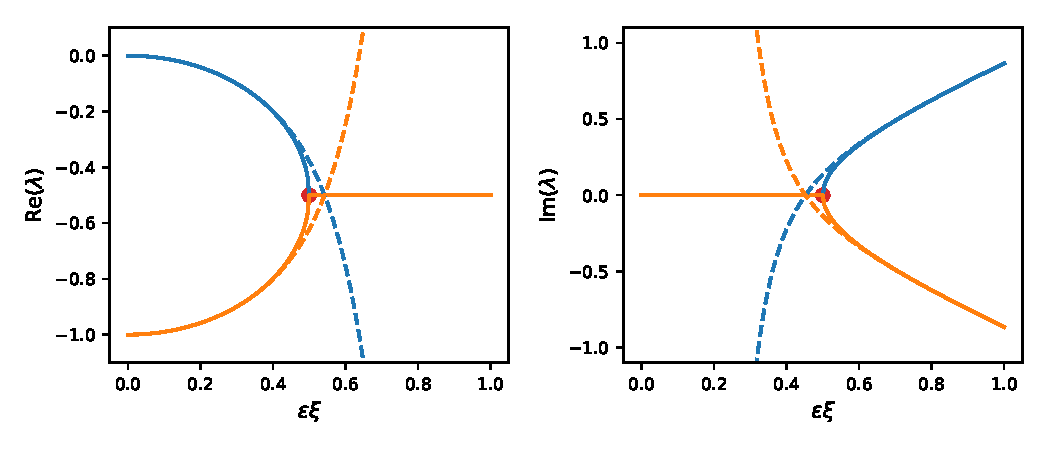
\includegraphics[width=.95\textwidth]{./Discussion/telegraph_eigenvalues.pdf}
    \caption{Tracé des valeurs propres du problème du télégraphe à un paramètre~\eqref{ext:pb:rescaled_telegraph} en fonction de $\eps\xi$, avec en bleu $\lambda_+$ et en orange $\lambda_-$ et leurs approximations en pointillées.}
    \label{ext:fig:telegraph_eig}
\end{figure}

Le principe de reconstruire une fonction $x \mapsto \widetilde{\omega}_{ij}(x)$ à partir de séries connues en $x \rightarrow 0$ et en $x \rightarrow \infty$ n'est pas nouveau. Une méthode de référence à cet effet est d'utiliser un approximant de Padé en deux points, dont la littérature est expensive~\cite{jones.1980.computation, jones.1983.two, baker.1996.pade, driscoll.2001.pade, tampos.2012.accurate}. Il faut néanmoins noter que ces constructions concernent seulement des fonctions à valeurs scalaires, et que la littérature pour les approximations de Padé de matrices semble se limiter à quelques articles d'André Draux,~\cite{draux.1984.pade,draux.1988.convergence}. Il n'est pas immédiat que l'approximation coefficient par coefficient présente des propriétés idéales (e.g. le changement de variable bien déterminé pour tout $\eps,\xi$). On espère néanmoins pouvoir utiliser ces méthodes pour construire des multiplicateurs de Fourier adaptés au problème du télégraphe.


